\documentclass[a4paper]{article}

% --- HỖ TRỢ TIẾNG VIỆT ---
\usepackage[utf8]{inputenc}      % đầu vào Unicode
\usepackage[T5]{fontenc}         % font T5 cho tiếng Việt
\usepackage[vietnamese]{babel}   % tiếng Việt

% --- CĂN LỀ & ĐỊNH DẠNG ---
\usepackage[left=2.5cm,right=2cm,top=2cm,bottom=2cm]{geometry} 
\setlength{\parindent}{0pt}

% --- VẼ HÌNH, ĐỒ HỌA ---
\usepackage{graphicx} 
\usepackage{tikz} 
\usepackage{float}


% --- KÝ HIỆU & MATH ---
\usepackage{array}
\usepackage{mathabx}
\usepackage{amsmath}
\usepackage{amsthm}
\newtheorem{definition}{Định nghĩa}
\usepackage{changepage} % Cho phép điều chỉnh lề

% --- TRANG TRÍ ---
\usepackage{wallpaper}
\usepackage{dashrule}
\usepackage[normalem]{ulem}
\usepackage{xcolor}

% --- DANH SÁCH, LIÊN KẾT ---
\usepackage{enumitem} 
\usepackage{hyperref}

% --- MÃ NGUỒN ---
\usepackage{listings}
\lstset{
  backgroundcolor=\color{gray!10},
  basicstyle=\ttfamily\small,
  frame=single,
  breaklines=true,
  captionpos=b,
  keywordstyle=\color{blue},
  commentstyle=\color{gray},
  stringstyle=\color{orange},
  columns=fullflexible,
  keepspaces=true
}

% --- KHÁC ---
\usepackage{caption}
\usepackage{scrextend}
\usepackage{longtable}
\usepackage{enumitem}
\usepackage[backend=biber]{biblatex}
\addbibresource{references.bib}


% --- FONT CỠ ---
\usepackage{titlesec}
\titleformat{\section}{\Large\bfseries}{\thesection}{1em}{}
\titleformat{\subsection}{\large\bfseries}{\thesubsection}{1em}{}

% Nếu cần chỉnh cỡ chữ chung:
\usepackage{anyfontsize}
\fontsize{16pt}{15.6pt}\selectfont
\linespread{1.2}





\lstset{
    language=[x86masm]Assembler,
    basicstyle=\ttfamily\footnotesize,
    keywordstyle=\color{blue},
    commentstyle=\color{gray},
    stringstyle=\color{red},
    numbers=left,
    numberstyle=\tiny,
    stepnumber=1,
    numbersep=5pt,
    backgroundcolor=\color{white},
    frame=single,
    tabsize=4,
    showspaces=false,
    showstringspaces=false
}

\begin{document}
	\newpage
	\begin{titlepage}
		\begin{tikzpicture}[remember picture,overlay,inner sep=0,outer sep=0]
			 \draw[blue!70!black,line width=4pt] 
			 ([xshift=1cm,yshift=1.5cm]current page.south west) coordinate (A)
			 -- ([xshift=-1cm,yshift=1.5cm]current page.south east) coordinate (B)
			 -- ([xshift=-1cm,yshift=-1.5cm]current page.north east) coordinate (C)
			 -- ([xshift=1cm,yshift=-1.5cm]current page.north west) coordinate (D)
			 -- cycle;
			 
			 % Viền gấp khúc trong
			 \draw ([yshift=0.5cm,xshift=-0.5cm]C)-- ([yshift=0.5cm,xshift=0.5cm]D)--
			 ([yshift=-0.5cm,xshift=0.5cm]D) --([yshift=-0.5cm,xshift=-0.5cm]D)
			 --([yshift=0.5cm,xshift=-0.5cm]A)--([yshift=0.5cm,xshift=0.5cm]A)
			 --([yshift=-0.5cm,xshift=0.5cm]A)-- ([yshift=-0.5cm,xshift=-0.5cm]B)
			 --([yshift=0.5cm,xshift=-0.5cm]B)--([yshift=0.5cm,xshift=0.5cm]B)
			 --([yshift=-0.5cm,xshift=0.5cm]C)--([yshift=-0.5cm,xshift=-0.5cm]C)
			 --([yshift=0.5cm,xshift=-0.5cm]C);
			 
			 \draw ([yshift=-0.3cm,xshift=0.3cm]C)-- ([yshift=-0.3cm,xshift=-0.3cm]D)--
			 ([yshift=0.3cm,xshift=-0.3cm]D) --([yshift=0.3cm,xshift=0.3cm]D)
			 --([yshift=-0.3cm,xshift=0.3cm]A)--([yshift=-0.3cm,xshift=-0.3cm]A)
			 --([yshift=0.3cm,xshift=-0.3cm]A)-- ([yshift=0.3cm,xshift=0.3cm]B)
			 --([yshift=-0.3cm,xshift=0.3cm]B)--([yshift=-0.3cm,xshift=-0.3cm]B)
			 --([yshift=0.3cm,xshift=-0.3cm]C)--([yshift=0.3cm,xshift=0.3cm]C)
			 --([yshift=-0.3cm,xshift=0.3cm]C);
			
		\end{tikzpicture}
		\begin{center}
			\vspace{2pt}
			
			\textbf{HỌC VIỆN CÔNG NGHỆ BƯU CHÍNH VIỄN THÔNG}
			
			\vspace{7pt}
			\textbf{KHOA CÔNG NGHỆ THÔNG TIN}
			
			\vspace{4pt}
			\hdashrule[0.5ex]{6cm}{1pt}{2mm 0.5mm}
		\end{center}
		
		\vspace{10pt}
		\begin{center}
			\includegraphics[scale=0.7]{ptit.png}
			
			\vspace{10pt}
			\fontsize{18pt}{17pt}\selectfont 
			\textbf{BÀI TẬP LỚN MÔN} 
			
			\vspace{7pt}
			\textbf{NHẬP MÔN TRÍ TUỆ NHÂN TẠO}
		\end{center}
		
		\vspace{10pt}
		\begin{flushleft}
			\fontsize{14pt}{17pt}\selectfont  
			\textbf{\textsl{ĐỀ TÀI}}
		\end{flushleft}
		\begin{center}
			\fontsize{18pt}{17pt}\selectfont 
			\textbf{\textrm{XÂY DỰNG HỆ THỐNG AI HỖ TRỢ VIẾT CV}}
		\end{center}
		
		\vspace{15pt}
		\begin{tabbing}
			\fontsize{16pt}{20pt}\selectfont
			\hspace{6cm} \= \hspace{5cm} \= \kill
			\textbf{Giáo viên hướng dẫn:} \> \textbf{TS.NGUYỄN THỊ MAI TRANG} \>\\ [6pt]
			\textbf{Nhóm học phần:} \> \textbf{14} \>\\ [6pt]
            \textbf{Nhóm bài tập lớn}\> \textbf{19} \>\\ [6pt]
			\textbf{Sinh viên:} \> \textbf{NGUYỄN QUANG DŨNG B22DCCN133} \>\\ [6pt]
            \textbf{} \> \textbf{NGUYỄN DUY HIẾU B22DCCN313} \>\\ [6pt]
            \textbf{} \> \textbf{BÙI MINH TÚ B22DCCN741} \>\\ [6pt]
			
		\end{tabbing}
		
		
		\vspace{14pt}
		\begin{center}
			\textbf{Hà Nội, 2025}
		\end{center}
	\end{titlepage}
	

\clearpage



\clearpage

% Mục lục
\tableofcontents

\clearpage

% Danh mục hình vẽ
\section*{DANH MỤC CÁC HÌNH VẼ}
\begin{itemize}
    \item Hình 1 - Tổng quan về cấu trúc GraphRAG và các công nghệ đi kèm theo thành phần \dotfill [số trang]
    \item Hình 2 - So sánh RAG và GraphRAG \dotfill [số trang]
    \item Hình 3 - Sơ đồ mô hình GAE \dotfill [số trang]
    \item Hình 4 - Sơ đồ luồng dữ liệu của hệ thống hỏi đáp pháp luật \dotfill [số trang]
\end{itemize}
\clearpage

% Danh mục bảng biểu
\section*{DANH MỤC CÁC BẢNG BIỂU}
\begin{itemize}
    \item Bảng 1 - Giá trị loss trong quá trình huấn luyện GAE \dotfill [số trang]
\end{itemize}
\clearpage

% Danh mục từ viết tắt
\section*{DANH MỤC CÁC TỪ VIẾT TẮT}
\begin{table}[h!]
\centering
\begin{tabular}{|p{2cm}|p{6cm}|p{6cm}|}
\hline
\textbf{Từ viết tắt} & \textbf{Thuật ngữ tiếng Anh/Giải thích} & \textbf{Thuật ngữ tiếng Việt/Giải thích} \\ \hline
GAE & Graph Auto-Encoder & Mã hóa đồ thị tự động \\ \hline
RAG & Retrieval-Augmented Generation & Tạo sinh tăng cường truy xuất \\ \hline
GNN & Graph Neural Network & Mạng nơ-ron đồ thị \\ \hline
LLM & Large Language Model & Mô hình ngôn ngữ lớn \\ \hline
\end{tabular}
\end{table}

\clearpage

%chuong 1:

\section{Tổng quan dự án}
\subsection{Giới thiệu bài toán}
Trong thời đại chuyển đổi số, nhu cầu tiếp cận thông tin pháp luật một cách nhanh chóng, chính xác và dễ hiểu ngày càng trở nên cấp thiết đối với mọi tầng lớp trong xã hội. Tuy nhiên, hệ thống văn bản pháp luật tại Việt Nam rất đồ sộ, phức tạp và thường xuyên thay đổi, gây khó khăn cho người dân, doanh nghiệp trong việc tra cứu, áp dụng đúng quy định. Các hệ thống hỏi đáp pháp luật truyền thống chủ yếu dựa trên tìm kiếm từ khóa, chưa khai thác được mối quan hệ phức tạp giữa các thực thể pháp lý, dẫn đến kết quả trả lời còn hạn chế về tính chính xác và khả năng suy luận.

Bài toán đặt ra là xây dựng một hệ thống AI có khả năng tiếp nhận câu hỏi tự nhiên của người dùng (input), truy xuất và tổng hợp thông tin từ kho dữ liệu pháp luật (bao gồm văn bản luật, các bài báo về luật pháp,các mối quan hệ giữa các thực thể pháp lý, v.v.), sau đó sinh ra câu trả lời tự động, chính xác, dễ hiểu (output). Dữ liệu đầu vào của hệ thống là các câu hỏi tiếng Việt về pháp luật và kho dữ liệu pháp luật đã được xử lý, chuẩn hóa dưới dạng văn bản và đồ thị tri thức. Đầu ra của hệ thống là các câu trả lời tự động, có thể kèm theo giải thích nguồn gốc, mối liên hệ giữa các điều khoản pháp luật liên quan.

\subsection{Mục đích và ý nghĩa}
\textbf{Mục đích:} Dự án hướng tới xây dựng một hệ thống AI hỗ trợ hỏi đáp pháp luật thông minh, tận dụng sức mạnh của các mô hình ngôn ngữ lớn (LLM) kết hợp với truy xuất tri thức từ đồ thị (Graph Retrieval-Augmented Generation - GraphRAG). Hệ thống giúp người dùng tra cứu thông tin pháp luật một cách nhanh chóng, chính xác, đồng thời có khả năng suy luận đa bước, giải thích các mối quan hệ giữa các điều khoản, văn bản pháp luật.

\textbf{Ý nghĩa:} Việc phát triển hệ thống này góp phần nâng cao nhận thức pháp luật, hỗ trợ doanh nghiệp và người dân tuân thủ pháp luật, đồng thời giảm tải cho các cơ quan tư vấn pháp lý truyền thống. Hệ thống còn là bước tiến quan trọng trong việc ứng dụng trí tuệ nhân tạo vào lĩnh vực pháp lý, thúc đẩy chuyển đổi số trong ngành luật tại Việt Nam.

\subsection{Công nghệ sử dụng}
Dự án ứng dụng các công nghệ hiện đại trong lĩnh vực trí tuệ nhân tạo và xử lý ngôn ngữ tự nhiên, bao gồm:
\begin{itemize}
    \item \textbf{Ngôn ngữ lập trình Python:} Ngôn ngữ chính được sử dụng để xây dựng toàn bộ hệ thống nhờ tính linh hoạt, thư viện phong phú và cộng đồng mạnh.
    \item \textbf{PyTorch:} Framework học sâu được sử dụng để xây dựng, huấn luyện và triển khai các mô hình AI như GAE.
    \item \textbf{Large Language Model (LLM):} Sử dụng các mô hình ngôn ngữ lớn để sinh câu trả lời tự nhiên, mạch lạc và phù hợp ngữ cảnh.
    \item \textbf{Graph Retrieval-Augmented Generation (GraphRAG):} Kết hợp truy xuất thông tin từ đồ thị tri thức pháp luật với khả năng sinh ngôn ngữ của LLM, giúp tăng cường độ chính xác và khả năng suy luận.
    \item \textbf{Graph Autoencoder (GAE):} Ứng dụng trong việc học biểu diễn các thực thể và quan hệ trong đồ thị pháp luật, hỗ trợ cho quá trình truy xuất và suy luận.
    \item \textbf{Cơ sở dữ liệu đồ thị (Neo4j):} Lưu trữ và quản lý dữ liệu pháp luật dưới dạng đồ thị, cho phép truy vấn các mối quan hệ phức tạp giữa các thực thể pháp lý.
    \item \textbf{MongoDB:} Lưu trữ dữ liệu văn bản gốc, bài báo, văn bản pháp luật trước khi xử lý và chuyển đổi sang đồ thị.
    \item \textbf{Flask:} Sử dụng Flask để xây dựng các API phục vụ giao tiếp giữa các thành phần của hệ thống và giao diện người dùng.
    \item \textbf{Streamlit:} Xây dựng giao diện web thân thiện, cho phép người dùng nhập câu hỏi và nhận phản hồi trực tiếp từ hệ thống.
\end{itemize}

\clearpage
\section{Cơ sở lý thuyết}
\subsection{Graph Retrieval-Augmented Generation}

\subsubsection{Giới thiệu về Retrieval-Augmented Generation (RAG)}
Retrieval-Augmented Generation (RAG) là một kỹ thuật kết hợp truy xuất thông tin và sinh nội dung để cải thiện hiệu suất các tác vụ xử lý ngôn ngữ tự nhiên ~\cite{Lewis2020RAG}. Trong RAG truyền thống, bộ truy xuất tìm kiếm thông tin từ nguồn dữ liệu văn bản $\mathcal{D} = \{d_1, d_2, \dots, d_n\}$ dựa trên truy vấn $q$, và bộ sinh tạo câu trả lời $y$ bằng cách tích hợp $q$ với thông tin truy xuất $R(q) \subseteq \mathcal{D}$. Quá trình này được mô tả bởi:
\begin{equation}
    y = \text{Generator}(q, R(q)),
\end{equation}
trong đó $R(q)$ là tập hợp các tài liệu liên quan được truy xuất ~\cite{Raffel2020T5}.

RAG truyền thống gặp hạn chế khi xử lý dữ liệu có quan hệ phức tạp, do thông tin được biểu diễn độc lập ~\cite{Chen2024GraphRAG}. GraphRAG khắc phục bằng cách sử dụng dữ liệu cấu trúc đồ thị để khai thác thông tin quan hệ, mở rộng khả năng suy luận đa bước và xử lý các tác vụ phức tạp.

\subsubsection{Định nghĩa và Đặc điểm của GraphRAG}
\begin{definition}[Đồ thị]
Một đồ thị $G = (V, E)$ bao gồm tập hợp các nút $V = \{v_1, v_2, \dots, v_n\}$ đại diện cho các thực thể và tập hợp các cạnh $E \subseteq V \times V$ biểu thị quan hệ giữa các thực thể.
\end{definition}

GraphRAG tích hợp dữ liệu đồ thị $G$ vào RAG, trong đó nguồn dữ liệu là $\mathcal{D}_G = \{G_1, G_2, \dots, G_m\}$, với mỗi $G_i$ là một đồ thị tri thức, đồ thị tài liệu, hoặc đồ thị miền cụ thể ~\cite{Liu2023GraphSurvey}. Quá trình GraphRAG được biểu diễn bằng:
\begin{equation}
    y = \text{Generator}(q, R_G(q)),
\end{equation}
trong đó $R_G(q)$ là tập hợp các nút, cạnh, hoặc đồ thị con liên quan được truy xuất từ $\mathcal{D}_G$ ~\cite{Chen2024GraphRAG}.

\subsubsection{Cấu trúc của GraphRAG}
GraphRAG bao gồm năm thành phần chính: Bộ xử lý truy vấn, Nguồn dữ liệu đồ thị, Bộ truy xuất, Bộ tổ chức, và Bộ sinh ~\cite{Chen2024GraphRAG}.
\begin{figure}[H]
    \centering
    \includegraphics[width=\textwidth]{gragStruct.png}
    \caption{Tổng quan về cấu trúc GraphRAG và các công nghệ đi kèm theo thành phần}

\end{figure}
\textbf{a.  Bộ xử lý truy vấn (Query Processor)}\\
Bộ xử lý truy vấn chuyển đổi truy vấn người dùng $q$ (thường ở dạng văn bản tự nhiên) thành một biểu diễn có cấu trúc $q_s$, phù hợp với dữ liệu đồ thị. Thành phần này thực hiện các chức năng như nhận diện thực thể (NER), trích xuất quan hệ (RE), cấu trúc hóa truy vấn, phân rã truy vấn, và mở rộng truy vấn ~\cite{Devlin2019BERT}.

\textbf{Ví dụ}: Với truy vấn $q = \text{``Thuốc nào điều trị sarcoma biểu mô và ảnh hưởng đến gen EZH2?''}$, bộ xử lý truy vấn:
\begin{itemize}
    \item Nhận diện $E_q = \{\text{sarcoma biểu mô}, \text{EZH2}\}$.
    \item Trích xuất $R_q = \{\text{điều trị}, \text{ảnh hưởng}\}$.
    \item Cấu trúc hóa thành truy vấn đồ thị $q_s$ với các nút $V_q = \{\text{thuốc}, \text{sarcoma biểu mô}, \text{EZH2}\}$ và các cạnh $E_q = \{(\text{thuốc}, \text{sarcoma biểu mô}, \text{điều trị}), (\text{thuốc}, \text{EZH2}, \text{ảnh hưởng})\}$.
\end{itemize}

Quá trình được mô tả bằng hàm ánh xạ:
\begin{equation}
    q_s = f_{\text{process}}(q; \theta),
\end{equation}
trong đó $\theta$ là tham số của mô hình (ví dụ: BERT cho NER). Xác suất một token $t_i$ thuộc thực thể $e_j$ là:
\begin{equation}
    P(e_j | t_i) = \text{softmax}(W \cdot \mathbf{h}_i + b),
\end{equation}
với $\mathbf{h}_i$ là nhúng token từ BERT ~\cite{Devlin2019BERT}.

\textbf{b.  Nguồn dữ liệu đồ thị (Graph Data Source)}\\
Nguồn dữ liệu đồ thị $\mathcal{D}_G = \{G_1, G_2, \dots, G_m\}$ bao gồm các đồ thị $G_i = (V_i, E_i)$, trong đó $V_i$ là tập hợp nút (thực thể) và $E_i$ là tập hợp cạnh (quan hệ). Các loại đồ thị bao gồm đồ thị tri thức, đồ thị tài liệu, và đồ thị sinh học ~\cite{Liu2023GraphSurvey}.

\textbf{Ví dụ}: Trong y học, $G$ là đồ thị tri thức với $V = \{\text{sarcoma biểu mô}, \text{EZH2}, \text{thuốc A}, \text{thuốc B}\}$ và $E = \{(\text{thuốc A}, \text{sarcoma biểu mô}, \text{điều trị}), (\text{thuốc B}, \text{EZH2}, \text{ảnh hưởng})\}$. Ma trận kề $A \in \mathbb{R}^{|V| \times |V|}$ được định nghĩa:
\begin{equation}
    A_{ij} = \begin{cases} 
        1 & \text{if } (v_i, v_j) \in E, \\
        0 & \text{otherwise.}
    \end{cases}
\end{equation}

Nguồn dữ liệu hỗ trợ truy xuất quan hệ với độ phức tạp lưu trữ $O(|V| + |E|)$ ~\cite{Zhang2022GraphIndex}.

\textbf{c.  Bộ truy xuất (Retriever)}\\
Bộ truy xuất tìm kiếm các phần tử liên quan $R_G(q_s) \subseteq V \cup E \cup \mathcal{G}$ từ $\mathcal{D}_G$ dựa trên $q_s$. Các kỹ thuật bao gồm liên kết thực thể, khớp quan hệ, duyệt đồ thị, và nhúng đồ thị bằng Graph Neural Networks (GNNs) ~\cite{Wu2020GNN}.

\textbf{Ví dụ}: Với $q_s$ chứa $E_q = \{\text{sarcoma biểu mô}, \text{EZH2}\}$, bộ truy xuất tìm các nút thuốc có cạnh liên quan. Nhúng nút $v_i$ từ GNN tại tầng $l+1$ là:
\begin{equation}
    \mathbf{h}_i^{(l+1)} = \sigma \left( \sum_{j \in \mathcal{N}(i)} \frac{1}{c_{ij}} \mathbf{h}_j^{(l)} W^{(l)} \right),
\end{equation}
với $\mathcal{N}(i)$ là tập lân cận, $c_{ij}$ là trọng số chuẩn hóa, và $\sigma$ là hàm kích hoạt. Độ tương đồng với nhúng truy vấn $\mathbf{h}_{q_s}$ được tính:
\begin{equation}
    \text{sim}(\mathbf{h}_{q_s}, \mathbf{h}_i) = \frac{\mathbf{h}_{q_s} \cdot \mathbf{h}_i}{\|\mathbf{h}_{q_s}\| \|\mathbf{h}_i\|}.
\end{equation}
Tập hợp $R_G(q_s)$ bao gồm các nút có $\text{sim} > \tau$ ~\cite{Wu2020GNN}.
\textbf{d.  Bộ tổ chức (Organizer)}\\
Bộ tổ chức tinh chỉnh $R_G(q_s)$ để tạo $R'_G(q_s)$, loại bỏ dư thừa và sắp xếp nội dung. Các kỹ thuật bao gồm cắt tỉa đồ thị, sắp xếp lại nội dung, và tóm tắt đồ thị ~\cite{Li2023GraphOrg}.

\textbf{Ví dụ}: Với $R_G(q_s)$ chứa nhiều nút thuốc, bộ tổ chức ưu tiên các nút có cả hai quan hệ ``điều trị'' và ``ảnh hưởng''. Điểm số nút $v_i$ là:
\begin{equation}
    \text{score}(v_i) = \alpha \cdot \text{sim}(\mathbf{h}_{q_s}, \mathbf{h}_i) + \beta \cdot C_B(v_i),
\end{equation}
với $C_B(v_i)$ là độ trung tâm giữa. Đồ thị con $G'$ được tối ưu:
\begin{equation}
    G' = \arg\max_{G' \subseteq G} \sum_{v_i \in V'} \text{score}(v_i) - \lambda |V'|.
\end{equation}

\textbf{e.  Bộ sinh (Generator)}\\
Bộ sinh tích hợp $q_s$ và $R'_G(q_s)$ để tạo câu trả lời $y$. Nhúng đồ thị $R'_G(q_s)$ được tổng hợp:
\begin{equation}
    \mathbf{h}_G = \text{READOUT}(\{\mathbf{h}_i \mid v_i \in R'_G(q_s)\}),
\end{equation}
với $\text{READOUT}$ là hàm tổng hợp (ví dụ: trung bình). Câu trả lời được sinh:
\begin{equation}
    y = \text{LLM}(q_s, \mathbf{h}_G; \phi),
\end{equation}
với $\phi$ là tham số của mô hình ngôn ngữ lớn (LLM) ~\cite{Brown2020GPT}.

\textbf{Ví dụ}: Với $R'_G(q_s)$ chứa các nút thuốc được tinh chỉnh, bộ sinh tạo: ``Thuốc A điều trị sarcoma biểu mô và ảnh hưởng đến gen EZH2 thông qua cơ chế ức chế''.

\textbf{f.  Tích hợp khung}\\
Khung GraphRAG hoạt động tuần tự:
\begin{equation}
    y = \text{Generator}(\text{Organizer}(\text{Retriever}(\text{Processor}(q), \mathcal{D}_G))),
\end{equation}
tối ưu hóa việc khai thác thông tin quan hệ và ngữ nghĩa, phù hợp với các ứng dụng đa dạng từ y học đến mạng xã hội ~\cite{Chen2024GraphRAG}.

\subsubsection{So sánh với RAG}
GraphRAG mở rộng RAG truyền thống bằng cách sử dụng cấu trúc đồ thị thay vì dữ liệu văn bản độc lập, mang lại nhiều ưu điểm nhưng cũng đi kèm với một số thách thức ~\cite{Chen2024GraphRAG}. Dưới đây là so sánh chi tiết giữa GraphRAG và RAG dựa trên các khía cạnh chính:\\
\textbf{a.  Cấu trúc dữ liệu\\}
Trong RAG, dữ liệu được lưu trữ dưới dạng văn bản $\mathcal{D} = \{d_1, d_2, \dots, d_n\}$, thường là các tài liệu hoặc đoạn văn, được biểu diễn bằng nhúng ngữ nghĩa (ví dụ: từ BERT hoặc DPR) ~\cite{Karpukhin2020DPR}. Quá trình truy xuất dựa trên độ tương đồng ngữ nghĩa:
\begin{equation}
    R(q) = \arg\max_{d_i \in \mathcal{D}} \text{sim}(\mathbf{h}_q, \mathbf{h}_{d_i}),
\end{equation}
trong đó $\mathbf{h}_q$ và $\mathbf{h}_{d_i}$ là nhúng của truy vấn và tài liệu.

Ngược lại, GraphRAG sử dụng đồ thị $\mathcal{D}_G = \{G_1, G_2, \dots, G_m\}$, với $G_i = (V_i, E_i)$, cho phép biểu diễn các thực thể và quan hệ ~\cite{Liu2023GraphSurvey}. Truy xuất trong GraphRAG dựa trên cấu trúc đồ thị, sử dụng nhúng GNN:
\begin{equation}
    R_G(q) = \{ v_i \in V \mid \text{sim}(\mathbf{h}_{q_s}, \mathbf{h}_i) > \tau \},
\end{equation}
với $\mathbf{h}_i$ được tính từ GNN ~\cite{Wu2020GNN}. Điều này cho phép GraphRAG khai thác các mối quan hệ phức tạp, ví dụ: tìm thuốc vừa ``điều trị'' sarcoma biểu mô vừa ``ảnh hưởng'' đến EZH2.

\textbf{b.  Khả năng truy xuất\\}
RAG truyền thống sử dụng các phương pháp truy xuất như DPR hoặc BM25, tập trung vào độ tương đồng ngữ nghĩa nhưng thiếu khả năng suy luận đa bước ~\cite{Lewis2020RAG}. Ví dụ, với truy vấn ``Thuốc nào điều trị sarcoma biểu mô và ảnh hưởng đến gen EZH2?'', RAG có thể trả về các tài liệu chứa từ khóa nhưng không đảm bảo kết nối hai quan hệ.

GraphRAG sử dụng các kỹ thuật duyệt đồ thị (BFS/DFS) và nhúng GNN để truy xuất các nút hoặc đồ thị con liên quan, hỗ trợ suy luận đa bước ~\cite{Chen2024GraphRAG}. Độ phức tạp truy xuất của GraphRAG phụ thuộc vào kích thước đồ thị, thường là $O(|V| + |E|)$ cho BFS, so với $O(n)$ của RAG (với $n$ là số tài liệu) ~\cite{Zhang2022GraphIndex}.

\textbf{c   Xử lý quan hệ phức tạp\\}
RAG truyền thống không hiệu quả trong việc xử lý các quan hệ phức tạp giữa các thực thể, do thiếu cấu trúc quan hệ ~\cite{Chen2024GraphRAG}. Ví dụ, RAG khó xác định một thuốc thỏa mãn cả hai quan hệ ``điều trị'' và ``ảnh hưởng'' trong cùng một truy vấn.

GraphRAG vượt trội nhờ khả năng biểu diễn quan hệ qua cạnh đồ thị và sử dụng GNN để tổng hợp thông tin lân cận ~\cite{Wu2020GNN}. Công thức nhúng GNN:
\begin{equation}
    \mathbf{h}_i^{(l+1)} = \sigma \left( \sum_{j \in \mathcal{N}(i)} \frac{1}{c_{ij}} \mathbf{h}_j^{(l)} W^{(l)} \right),
\end{equation}
cho phép GraphRAG nắm bắt các mối quan hệ cấp cao, như đường đi giữa các nút trong đồ thị tri thức y học, pháp luật.\\
\textbf{d.  Hiệu quả tính toán\\}
RAG truyền thống có chi phí tính toán thấp hơn, do chỉ yêu cầu nhúng văn bản và tìm kiếm tuyến tính ~\cite{Karpukhin2020DPR}. Tuy nhiên, GraphRAG đòi hỏi tài nguyên tính toán cao hơn, đặc biệt khi xử lý đồ thị lớn với GNN, với độ phức tạp $O(|V| \cdot d^2)$ cho mỗi tầng GNN (với $d$ là kích thước nhúng) ~\cite{Wu2020GNN}.
\textbf{Ứng dụng} RAG phù hợp với các tác vụ đơn giản như trả lời câu hỏi dựa trên tài liệu, nhưng kém hiệu quả trong các lĩnh vực yêu cầu quan hệ phức tạp, như phân tích sinh học hoặc mạng xã hội ~\cite{Lewis2020RAG}. GraphRAG được thiết kế cho các ứng dụng đòi hỏi suy luận quan hệ, ví dụ: phân tích mạng sinh học để tìm thuốc hoặc dự đoán liên kết xã hội ~\cite{Chen2024GraphRAG}.
\textbf{Bảng so sánh}:
\begin{center}
\begin{tabular}{|c|c|c|}
\hline
\textbf{Tiêu chí} & \textbf{RAG} & \textbf{GraphRAG} \\
\hline
Cấu trúc dữ liệu & Văn bản $\mathcal{D}$ & Đồ thị $\mathcal{D}_G$ \\
Khả năng truy xuất & Ngữ nghĩa, đơn bước & Quan hệ, đa bước \\
Xử lý quan hệ & Kém & Tốt \\
Hiệu quả tính toán & Cao & Thấp hơn \\
Ứng dụng & Trả lời câu hỏi đơn giản & Phân tích quan hệ phức tạp \\
\hline
\end{tabular}
\end{center}
\begin{figure}[H]
    \centering
    \includegraphics[width=\textwidth]{gragvsrag.png}
    \caption{So sánh RAG và GraphRAG}

\end{figure}

\textbf{Kết luận}: GraphRAG vượt trội so với RAG trong việc xử lý dữ liệu có quan hệ phức tạp nhờ cấu trúc đồ thị và các kỹ thuật như GNN, nhưng yêu cầu tài nguyên tính toán cao hơn. Sự lựa chọn giữa RAG và GraphRAG phụ thuộc vào yêu cầu ứng dụng ~\cite{Chen2024GraphRAG}.
\subsubsection{Ứng dụng và Thách thức}
GraphRAG hỗ trợ nhiều ứng dụng, từ trả lời câu hỏi trên đồ thị tri thức đến phân tích dữ liệu sinh học. Tuy nhiên, các thách thức bao gồm:
\begin{itemize}
    \item \textbf{Định dạng đa dạng}: Xử lý các loại đồ thị khác nhau ($G$ có thể là đồ thị tri thức, đồ thị tài liệu, v.v.).
    \item \textbf{Suy luận đa bước}: Yêu cầu duyệt đồ thị với độ phức tạp $O(|V| + |E|)$.
    \item \textbf{Tính đặc thù theo miền}: Thiết kế riêng cho từng miền ứng dụng.
\end{itemize}

\subsection{Graph Autoencoder (GAE)}

Graph Autoencoder (GAE) là một mô hình học không giám sát trên đồ thị, được phát triển nhằm học biểu diễn (embedding) của các đỉnh trong đồ thị sao cho có thể khôi phục lại cấu trúc đồ thị đầu vào. Ý tưởng xuất phát từ mô hình autoencoder truyền thống, nhưng được điều chỉnh để làm việc hiệu quả với dữ liệu phi Euclid như đồ thị.

\subsubsection{Kiến trúc tổng thể của GAE}

Mô hình GAE bao gồm hai thành phần chính:

\begin{itemize}
  \item \textbf{Encoder:} Dùng để ánh xạ đặc trưng đỉnh ban đầu (hoặc đơn vị) và cấu trúc đồ thị thành không gian tiềm ẩn. Thông thường, encoder được xây dựng dựa trên mạng nơ-ron tích chập trên đồ thị (Graph Convolutional Networks - GCN) ~\cite{kipf2016semi}.
  \item \textbf{Decoder:} Nhận đầu vào là biểu diễn tiềm ẩn và tái tạo lại ma trận kề của đồ thị. Một decoder cơ bản dùng tích vô hướng giữa các vector biểu diễn đỉnh
  
\end{itemize}
\begin{figure}[H]
    \centering
    \includegraphics[width=0.8\textwidth]{gae_struct.png}
    \caption{Sơ đồ mô hình GAE }
\end{figure}

\textbf{a.  Encoder}\\
Encoder có nhiệm vụ biến đổi đặc trưng đầu vào $\mathbf{X} \in \mathbb{R}^{n \times d}$ và cấu trúc đồ thị (thông qua ma trận kề $\mathbf{A} \in \{0,1\}^{n \times n}$) thành biểu diễn tiềm ẩn $\mathbf{Z} \in \mathbb{R}^{n \times d'}$ cho các đỉnh.

Một encoder phổ biến sử dụng mạng nơ-ron tích chập trên đồ thị (Graph Convolutional Network - GCN) như được đề xuất trong ~\cite{kipf2016semi}. Với một tầng GCN, công thức lan truyền được định nghĩa như sau:
\begin{equation}
\mathbf{H}^{(l+1)} = \sigma\left( \tilde{\mathbf{D}}^{-\frac{1}{2}} \tilde{\mathbf{A}} \tilde{\mathbf{D}}^{-\frac{1}{2}} \mathbf{H}^{(l)} \mathbf{W}^{(l)} \right)
\end{equation}.



trong đó:

\begin{itemize}
  \item $\tilde{\mathbf{A}} = \mathbf{A} + \mathbf{I}_n$ là ma trận kề với liên kết tự thân,
  \item $\tilde{\mathbf{D}}$ là ma trận bậc tương ứng với $\tilde{\mathbf{A}}$,
  \item $\mathbf{W}^{(l)}$ là trọng số học được tại tầng $l$,
  \item $\sigma(\cdot)$ là hàm kích hoạt, thường là ReLU,
  \item $\mathbf{H}^{(0)} = \mathbf{X}$ là đặc trưng đầu vào.
\end{itemize}

Với hai tầng GCN, biểu diễn tiềm ẩn của đỉnh được tính như sau:

\begin{equation}
\mathbf{Z} = \text{GCN}(\mathbf{X}, \mathbf{A}) = \tilde{\mathbf{A}} \cdot \text{ReLU}(\tilde{\mathbf{A}} \cdot \mathbf{X} \cdot \mathbf{W}^{(0)}) \cdot \mathbf{W}^{(1)}
\end{equation}
Trong trường hợp của \textit{Variational GAE} (VGAE) ~\cite{kipf2016variational}, encoder được mở rộng để sinh ra hai đầu ra: trung bình $\boldsymbol{\mu}$ và phương sai $\boldsymbol{\sigma}$ để mô hình hóa phân phối xác suất:

\begin{equation}
\mathbf{z}_i = \boldsymbol{\mu}_i + \boldsymbol{\sigma}_i \odot \boldsymbol{\epsilon}, \quad \boldsymbol{\epsilon} \sim \mathcal{N}(0, \mathbf{I})
\end{equation}
\textbf{b.  Decoder}\\
Decoder có nhiệm vụ tái tạo ma trận kề $\hat{\mathbf{A}}$ từ biểu diễn tiềm ẩn $\mathbf{Z}$. Cách đơn giản và phổ biến nhất để thực hiện việc này là sử dụng tích vô hướng giữa các embedding:

\begin{equation}
\hat{A}_{ij} = \sigma(\mathbf{z}_i^\top \mathbf{z}_j)
\end{equation}

Trong đó $\sigma(\cdot)$ là hàm sigmoid, và $\hat{A}_{ij}$ biểu diễn xác suất tồn tại cạnh giữa đỉnh $i$ và đỉnh $j$.  

Ngoài ra, decoder có thể được mở rộng thành mạng neural đa lớp hoặc dùng attention để tăng khả năng mô hình hóa các cấu trúc phức tạp hơn.

\subsubsection{Hàm mất mát}

GAE sử dụng hàm mất mát là cross-entropy giữa ma trận kề thực tế và ma trận dự đoán:

\begin{equation}
\mathcal{L} = -\sum_{(i,j) \in \Omega^+ \cup \Omega^-} \left[ A_{ij} \log \hat{A}_{ij} + (1 - A_{ij}) \log (1 - \hat{A}_{ij}) \right]
\end{equation}

trong đó:
\begin{itemize}
  \item $\Omega^+$ là tập các cặp đỉnh có cạnh thật,
  \item $\Omega^-$ là tập các cặp đỉnh không có cạnh, được chọn ngẫu nhiên (negative sampling).
\end{itemize}

Đối với mô hình VGAE, hàm mất mát được mở rộng để bao gồm thêm sai khác KL giữa phân phối ẩn và phân phối chuẩn:

\begin{equation}
\mathcal{L}_{\text{VGAE}} = \mathbb{E}_{q(\mathbf{Z}|\mathbf{X}, \mathbf{A})}[\log p(\mathbf{A}|\mathbf{Z})] - \text{KL}[q(\mathbf{Z}|\mathbf{X}, \mathbf{A}) \,\|\, p(\mathbf{Z})]
\end{equation}

Trong đó $p(\mathbf{Z})$ là phân phối chuẩn hoá $\mathcal{N}(0, \mathbf{I})$ và $q(\mathbf{Z}|\mathbf{X}, \mathbf{A})$ là phân phối xác suất sinh bởi encoder.



\subsubsection{Quy trình huấn luyện}

Mục tiêu của GAE là tối thiểu hóa sai số tái tạo giữa ma trận kề thực $A$ và ma trận được dự đoán $\hat{A}$. Hàm mất mát phổ biến nhất là binary cross-entropy:
\begin{equation}
\mathcal{L} = - \sum_{i,j} [A_{ij} \log \hat{A}_{ij} + (1 - A_{ij}) \log (1 - \hat{A}_{ij})]
\end{equation}

Trong trường hợp đồ thị lớn và thưa, thường sử dụng sampling âm để giảm chi phí tính toán. Tập dương là các cạnh có thật trong đồ thị, trong khi tập âm là các cặp đỉnh không kết nối được lấy ngẫu nhiên.

Huấn luyện GAE bao gồm các bước:

\begin{enumerate}
  \item Khởi tạo đặc trưng đỉnh $X$ và ma trận kề $A$
  \item Truyền $X$ qua encoder để thu được biểu diễn $Z$
  \item Tính $\hat{A}$ từ $Z$ qua decoder
  \item Tính toán hàm mất mát và cập nhật tham số qua lan truyền ngược
\end{enumerate}

\subsubsection{Biến thể của GAE}

\textbf{a.  Variational Graph Autoencoder (VGAE)} ~\cite{kipf2016variational}:  
Thay vì học vector $Z$ cố định, mô hình học phân phối xác suất $q(z|x)$ và lấy mẫu từ phân phối này. Hàm mất mát là ELBO:
\begin{equation}
\mathcal{L}_{\text{VGAE}} = \mathbb{E}_{q(Z|X,A)}[\log p(A|Z)] - \text{KL}[q(Z|X,A) \Vert p(Z)]
\end{equation}
Trong đó $q$ là phân phối Gaussian có trung bình và phương sai học được từ GCN.

\textbf{b.  Adversarially Regularized GAE (ARGA)} ~\cite{pan2018arga}:  
Kết hợp GAE với huấn luyện đối kháng (GAN) để làm biểu diễn gần với phân phối chuẩn thông qua discriminator. Điều này giúp giảm overfitting và tăng khả năng tổng quát.

\textbf{c.  Marginalized GAE (MGAE)} ~\cite{wang2017mgae}:  
Encoder được xây dựng từ autoencoder tuyến tính, thêm nhiễu vào đầu vào để tăng tính kháng nhiễu, sau đó marginalize qua nhiễu. Phù hợp với bài toán phân cụm.

\textbf{d.  GraphVAE và Graphite:}  
Các mô hình mở rộng nhằm sinh đồ thị mới từ không gian tiềm ẩn, đặc biệt phù hợp với ứng dụng sinh phân tử và thiết kế mạng.

\subsubsection{Ứng dụng}

Các ứng dụng điển hình của GAE bao gồm:

\begin{itemize}
  \item \textbf{Dự đoán liên kết (Link Prediction)}: Dự đoán các cạnh tiềm năng bằng cách tính xác suất kết nối giữa các cặp đỉnh trong không gian tiềm ẩn.
  \item \textbf{Phân cụm/Phân loại đỉnh}: Biểu diễn $Z$ có thể dùng làm đầu vào cho các mô hình học máy khác để thực hiện phân loại bán giám sát.
  \item \textbf{Sinh đồ thị (Graph Generation)}: Đặc biệt ứng dụng trong sinh phân tử, cấu trúc hóa học.
  \item \textbf{Phát hiện bất thường}: Những đỉnh/cạnh có lỗi tái tạo cao có thể được xem là bất thường.
\end{itemize}

\subsubsection{Hạn chế và hướng phát triển}

\begin{itemize}
  \item GAE không dễ mở rộng với đồ thị lớn do tính phức tạp $O(n^2)$ khi tính tích vô hướng.
  \item Mô hình decoder đơn giản có thể không đủ mạnh để tái tạo cấu trúc phức tạp.
  \item Vấn đề ``over-smoothing'' trong encoder nhiều tầng vẫn là một thách thức.
  \item Việc mở rộng sang đồ thị dị thể, động, hoặc có thuộc tính cạnh phức tạp đang là hướng nghiên cứu mới.
\end{itemize}

Một số hướng cải tiến đang được quan tâm bao gồm:
\begin{itemize}
  \item Sử dụng encoder có attention (GAT), hoặc Transformer cho đồ thị.
  \item Kết hợp học tương phản (contrastive learning) để tăng cường biểu diễn.
  \item Tích hợp dữ liệu thuộc tính phức tạp hoặc nhiều loại nút/cạnh.
\end{itemize}


\newpage
\section{Phân tích và thiết kế dự án}
\subsection{Phân tích dự án}
\subsubsection{Phân tích yêu cầu hệ thống}
Hệ thống hướng tới mục tiêu hỗ trợ người dùng tra cứu, hỏi đáp pháp luật một cách tự động, nhanh chóng và chính xác. Dưới đây là các yêu cầu chính:

\textbf{Yêu cầu chức năng:}
\begin{itemize}
    \item Nhận câu hỏi tiếng Việt về pháp luật từ người dùng qua giao diện web.
    \item Xử lý truy vấn, truy xuất thông tin pháp luật liên quan từ cơ sở dữ liệu.
    \item Sinh câu trả lời tự động, trả về cho người dùng.
    \item Chuẩn bị, thu thập, xử lý và xây dựng dữ liệu pháp luật phục vụ cho hệ thống hỏi đáp.
\end{itemize}
\textbf{Yêu cầu phi chức năng:}
\begin{itemize}
    \item Thời gian phản hồi nhanh, đảm bảo trải nghiệm người dùng.
    \item Độ chính xác cao trong việc truy xuất và sinh câu trả lời.
    \item Giao diện đơn giản, dễ sử dụng, phù hợp với nhiều đối tượng.
    \item Hệ thống dễ dàng mở rộng, bảo trì và tích hợp thêm dữ liệu mới.
\end{itemize}

\subsubsection{Phân tích luồng hoạt động chính}
Quy trình hoạt động của hệ thống được mô tả như sau:
\begin{enumerate}
    \item Giai đoạn chuẩn bị dữ liệu: Thu thập, chuẩn hóa, trích xuất thực thể/quan hệ từ văn bản pháp luật, xây dựng đồ thị tri thức (thực hiện bởi các script như make\_data.py, insert\_graph\_db.py).
    \item Giai đoạn hỏi đáp: Người dùng nhập câu hỏi về pháp luật vào giao diện web (Streamlit).
    \item Giao diện gửi câu hỏi đến API backend (Flask).
    \item Backend tiếp nhận câu hỏi, chuyển tới module AI để xử lý.
    \item Module AI thực hiện truy xuất thông tin liên quan từ đồ thị tri thức (Neo4j) và dữ liệu văn bản (MongoDB).
    \item Mô hình ngôn ngữ lớn (LLM) sinh câu trả lời dựa trên thông tin truy xuất được.
    \item Backend trả về câu trả lời cho giao diện web để hiển thị cho người dùng.
\end{enumerate}

\subsubsection{Phân tích dữ liệu đầu vào, đầu ra và mô hình hóa dữ liệu}
Dữ liệu là nền tảng quan trọng của hệ thống hỏi đáp pháp luật. Việc phân tích và mô hình hóa dữ liệu giúp đảm bảo hệ thống hoạt động hiệu quả, truy xuất và sinh câu trả lời chính xác.

\textbf{Dữ liệu đầu vào:}
\begin{itemize}
    \item Câu hỏi tiếng Việt do người dùng nhập vào giao diện web, thường là các thắc mắc về quy định pháp luật, điều khoản, quyền và nghĩa vụ.
    \item Kho dữ liệu pháp luật gồm: văn bản luật, các bài báo liên quan, dữ liệu đã được trích xuất thực thể và quan hệ từ các nguồn này.
\end{itemize}

\textbf{Dữ liệu đầu ra:}
\begin{itemize}
    \item Câu trả lời tự động, ngắn gọn, chính xác, có thể kèm theo giải thích nguồn gốc hoặc mối liên hệ giữa các điều khoản pháp luật liên quan.
\end{itemize}

\textbf{Mô hình hóa dữ liệu:}
\begin{itemize}
    \item \textbf{Các thực thể chính:} Luật, Điều, Khoản, Thực thể pháp lý (ví dụ: cá nhân, tổ chức, cơ quan ban hành), Quan hệ pháp lý (ví dụ: ban hành, quy định, áp dụng).
    \item \textbf{Lưu trữ dữ liệu văn bản:} Các văn bản luật, bài báo, dữ liệu gốc được lưu trữ trong MongoDB dưới dạng các collection, thuận tiện cho việc truy xuất và cập nhật.
    \item \textbf{Đồ thị tri thức pháp luật:} Dữ liệu đã được trích xuất thực thể và quan hệ sẽ được xây dựng thành đồ thị tri thức và lưu trữ trong Neo4j. Mỗi node đại diện cho một thực thể pháp lý, mỗi edge đại diện cho một quan hệ pháp lý giữa các thực thể.
\end{itemize}

Việc mô hình hóa dữ liệu như trên giúp hệ thống dễ dàng truy xuất thông tin liên quan, hỗ trợ quá trình suy luận và sinh câu trả lời chính xác cho người dùng.
\subsection{Thiết kế dự án}
\subsubsection{Thiết kế kiến trúc hệ thống}
Hệ thống được thiết kế theo mô hình client-server với các thành phần chính như sau:
\begin{itemize}
    \item \textbf{Module xử lý và chuẩn bị dữ liệu:} Bao gồm các script như make\_data.py (thu thập, chuẩn hóa, trích xuất thực thể/quan hệ, lưu vào MongoDB) và insert\_graph\_db.py (xây dựng, cập nhật đồ thị tri thức trong Neo4j).
    \item \textbf{Giao diện web (Streamlit):} Cho phép người dùng nhập câu hỏi và hiển thị câu trả lời.
    \item \textbf{API backend (Flask):} Nhận câu hỏi từ giao diện, chuyển tiếp truy vấn đến các thành phần xử lý và trả về kết quả.
    \item \textbf{LLM1 (trích xuất thực thể/quan hệ):} Mô hình ngôn ngữ lớn đầu tiên, đảm nhiệm vai trò trích xuất thực thể và quan hệ từ câu hỏi của người dùng để hỗ trợ truy xuất thông tin chính xác trong đồ thị tri thức.
    \item \textbf{Mô hình Graph AutoEncoder (GAE):} Học biểu diễn (embedding) cho các đỉnh trong đồ thị tri thức pháp luật, hỗ trợ truy xuất và suy luận các quan hệ pháp lý.
    \item \textbf{LLM2 (sinh câu trả lời):} Mô hình ngôn ngữ lớn thứ hai, đảm nhiệm vai trò tổng hợp, diễn giải và sinh ra câu trả lời tự động, tự nhiên, dễ hiểu cho người dùng dựa trên thông tin đã truy xuất được.
    \item \textbf{Cơ sở dữ liệu:} Lưu trữ văn bản pháp luật, dữ liệu đã trích xuất (MongoDB) và đồ thị tri thức (Neo4j).
\end{itemize}
\textbf{Mô tả luồng dữ liệu:} Khi người dùng gửi câu hỏi, dữ liệu được truyền từ giao diện web đến backend, LLM1 sẽ trích xuất thực thể/quan hệ từ câu hỏi, truy xuất thông tin từ cơ sở dữ liệu, embedding và suy luận bằng GAE, sau đó LLM2 sinh câu trả lời và trả về cho người dùng. Dữ liệu nền tảng được chuẩn bị, cập nhật định kỳ qua các script xử lý dữ liệu.

\subsubsection{Thiết kế chi tiết các module}
\textbf{Module xử lý và chuẩn bị dữ liệu:} 
\begin{itemize}
    \item \textbf{make\_data.py:} Thu thập dữ liệu pháp luật từ các nguồn (web, văn bản, bài báo), chuẩn hóa lưu trữ vào MongoDB hoặc các file JSON ở local.
    \item \textbf{insert\_graph\_db.py:} Đọc dữ liệu từ MongoDB hoặc các file JSON ở local, xây dựng và cập nhật đồ thị tri thức pháp luật trong Neo4j, đảm bảo dữ liệu sẵn sàng cho truy xuất AI.
\end{itemize}
\textbf{Giao diện người dùng (Streamlit):}
\begin{itemize}
    \item Giao diện đơn giản với một ô nhập câu hỏi và khu vực hiển thị câu trả lời.
    \item Khi người dùng nhập câu hỏi và gửi, hệ thống sẽ hiển thị câu trả lời trả về từ backend.
\end{itemize}
\textbf{API backend (Flask):}
\begin{itemize}
    \item Cung cấp endpoint nhận câu hỏi từ giao diện web (POST /api/chatbot).
    \item Nhận dữ liệu JSON chứa câu hỏi, chuyển tiếp tới LLM1, GAE, LLM2 và trả về dữ liệu JSON chứa câu trả lời.
\end{itemize}
\textbf{LLM1 (trích xuất thực thể/quan hệ):}
\begin{itemize}
    \item \textbf{Vai trò:} Nhận câu hỏi từ người dùng, sử dụng mô hình ngôn ngữ lớn để trích xuất các thực thể và quan hệ quan trọng, phục vụ cho việc truy xuất thông tin chính xác trong đồ thị tri thức.
    \item \textbf{Luồng dữ liệu:} Đầu vào là câu hỏi của người dùng, đầu ra là danh sách thực thể và quan hệ được trích xuất.
\end{itemize}
\textbf{Mô hình Graph AutoEncoder (GAE):}
\begin{itemize}
    \item \textbf{Vai trò:} Học biểu diễn (embedding) cho các đỉnh trong đồ thị tri thức pháp luật, giúp mô hình hóa quan hệ giữa các thực thể pháp lý và hỗ trợ quá trình truy xuất, suy luận.
    \item \textbf{Kiến trúc:} Mô hình gồm hai lớp GCN (Graph Convolutional Network) liên tiếp.
    \item \textbf{Luồng dữ liệu:} Đầu vào là đặc trưng các đỉnh và danh sách cạnh, đầu ra là embedding các đỉnh và dự đoán tồn tại cạnh.
\end{itemize}
\textbf{LLM2 (sinh câu trả lời):}
\begin{itemize}
    \item \textbf{Vai trò:} Sau khi truy xuất được thông tin liên quan, LLM2 tổng hợp, diễn giải và sinh ra câu trả lời tự động, tự nhiên, dễ hiểu cho người dùng.
    \item \textbf{Luồng dữ liệu:} Đầu vào là thông tin pháp luật đã truy xuất và câu hỏi gốc, đầu ra là câu trả lời hoàn chỉnh, mạch lạc, có thể kèm giải thích nguồn gốc hoặc mối liên hệ giữa các điều khoản pháp luật.
\end{itemize}

\subsubsection{Sơ đồ luồng dữ liệu và hoạt động}
Luồng dữ liệu của hệ thống được mô tả như sau:
\begin{itemize}
    \item Giai đoạn chuẩn bị dữ liệu: Các script make\_data.py và insert\_graph\_db.py thu thập, xử lý, xây dựng dữ liệu nền tảng cho hệ thống.
    \item Giai đoạn hỏi đáp: Người dùng nhập câu hỏi trên giao diện web (Streamlit), câu hỏi được gửi tới API backend (Flask), backend chuyển câu hỏi tới module AI để truy xuất thông tin và sinh câu trả lời, kết quả trả về giao diện web.
\end{itemize}
\begin{figure}[H]
    \centering
    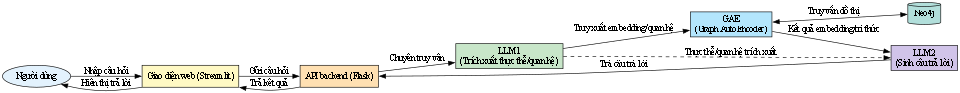
\includegraphics[width=1.05\textwidth]{dataflow.png}
    \caption{Sơ đồ luồng dữ liệu của hệ thống hỏi đáp pháp luật}
\end{figure}

\subsubsection{Các quyết định thiết kế và lý do lựa chọn}
\begin{itemize}
    \item Sử dụng Python vì tính linh hoạt, thư viện AI mạnh và cộng đồng hỗ trợ lớn.
    \item PyTorch được lựa chọn để xây dựng và huấn luyện các mô hình AI như GAE, LLM nhờ khả năng tùy biến và hiệu năng tốt.
    \item Flask phù hợp để xây dựng API backend đơn giản, dễ tích hợp với các thành phần khác.
    \item Streamlit giúp phát triển giao diện web nhanh chóng, thân thiện với người dùng.
    \item MongoDB lưu trữ dữ liệu phi cấu trúc (văn bản, bài báo), còn Neo4j phù hợp cho dữ liệu đồ thị tri thức pháp luật.
    \item Việc kết hợp LLM, GraphRAG, GAE giúp hệ thống tăng khả năng hiểu ngữ nghĩa, truy xuất và suy luận pháp lý, nâng cao chất lượng câu trả lời.
    \item Các script xử lý dữ liệu giúp hệ thống luôn có dữ liệu nền tảng sạch, có cấu trúc, sẵn sàng cho truy xuất và hỏi đáp.
\end{itemize}

\newpage
\section{Cài đặt và kiểm thử}
\subsection{Cấu trúc mã nguồn}

\begin{verbatim}
thuc_tap_co_so/
├── baocao.tex
├── requirements.txt //các thư viện cần thiết
├── README.md //tổng quan về dự án
├── make_data/
│ ├── make_data.py //thu thập, chuẩn hóa, trích xuất thực thể/quan hệ, lưu vào MongoDB
│ ├── insert_graph_db.py //đọc dữ liệu từ MongoDB hoặc các file JSON ở local, xây dựng và cập nhật đồ thị tri thức trong Neo4j
│ └── data/ //dữ liệu đã được chuẩn hóa và trích xuất
├── src/
│ ├── ai_model/
│ │ ├── gae/
│ │ │ ├── train.py //train model gae
│ │ │ ├── test.py //test model gae
│ │ │ ├── model.py //model gae
│ │ │ └── gae.torch //model gae đã được train
│ │ ├── llm/
│ │ │ └── model.py //model llm call api gemini về
│ │ └── retrieve.py //khối truy xuất thông tin từ graphdb
│ └── web_app/
│ ├── stremlit_web.py //giao diện web
│ └── back_end/
│ └── chatbot_api.py //api backend
\end{verbatim}



\subsection{Cài đặt và train model GAE}
\subsubsection{Cài đặt model GAE}
Mô hình Graph AutoEncoder (GAE) được xây dựng bằng thư viện PyTorch Geometric, sử dụng hai lớp GCN để học biểu diễn (embedding) cho các đỉnh trong đồ thị tri thức pháp luật.
\textbf{Kiến trúc mô hình:}
\begin{itemize}
\item \textbf{Lớp encoder1:} GCNConv đầu vào, ánh xạ từ số chiều đặc trưng ban đầu (\texttt{input\dim}) sang không gian ẩn (\texttt{hidden\_dim}).
\item \textbf{Lớp encoder2:} GCNConv tiếp theo, ánh xạ từ không gian ẩn sang không gian embedding (\texttt{embedding\dim}).
\item \textbf{Hàm encode:} Truyền dữ liệu qua hai lớp GCN, sử dụng hàm kích hoạt ReLU ở lớp đầu.
\item \textbf{Hàm decode:} Dự đoán khả năng tồn tại cạnh giữa hai đỉnh dựa trên tích vô hướng của embedding.
\item \textbf{Hàm forward:} Kết hợp encode và decode để huấn luyện và đánh giá mô hình.
\end{itemize}
\textbf{Tham số cấu hình:}
\begin{itemize}
\item \texttt{input\dim}: Số chiều đặc trưng đầu vào của mỗi node. Trong hệ thống này, sử dụng one-hot encoding nên \texttt{input\_dim} = số lượng node trong đồ thị.
\item \texttt{hidden\dim}: Số chiều không gian ẩn, thường đặt là 16.
\item \texttt{embedding\dim}: Số chiều vector embedding đầu ra, thường đặt là 8.
\item \texttt{epochs}: Số vòng lặp huấn luyện, thường đặt là 200.
\item \texttt{optimizer}: Adam, learning rate 0.01.
\end{itemize}
\textbf{Ví dụ khởi tạo mô hình:}
\begin{lstlisting}[language=python]
input_dim = features.size(1) # Số node (one-hot)
hidden_dim = 16
embedding_dim = 8
model = GAE(input_dim, hidden_dim, embedding_dim)
optimizer = torch.optim.Adam(model.parameters(), lr=0.01)
\end{lstlisting}
\subsubsection{Train model GAE}

Dữ liệu đầu vào cho quá trình huấn luyện mô hình GAE gồm:
\begin{itemize}
    \item \textbf{Số node:} 3000 (mỗi node đại diện cho một thực thể pháp lý, được mã hóa one-hot).
    \item \textbf{Số cạnh (edge):} 4000 (mỗi cạnh đại diện cho một quan hệ pháp lý giữa hai thực thể).
\end{itemize}

\textbf{Chia tập train/validation:}
\begin{itemize}
    \item Toàn bộ 4000 cạnh được trộn ngẫu nhiên.
    \item 80\% số cạnh (3200 cạnh) dùng cho huấn luyện (train), 20\% còn lại (800 cạnh) dùng cho kiểm thử (validation).
    \item Việc chia này đảm bảo các cạnh trong tập train và validation không trùng lặp, giúp đánh giá khả năng tổng quát hóa của mô hình.
\end{itemize}

\textbf{Quy trình huấn luyện:}
\begin{itemize}
    \item Sử dụng PyTorch Geometric để xây dựng và huấn luyện mô hình GAE với các tham số:
    \begin{itemize}
        \item \texttt{input\_dim} = 3000 (số node, do dùng one-hot encoding)
        \item \texttt{hidden\_dim} = 16
        \item \texttt{embedding\_dim} = 8
        \item \texttt{epochs} = 200
        \item \texttt{optimizer}: Adam, learning rate 0.01
    \end{itemize}
    \item Trong mỗi epoch, mô hình được huấn luyện trên tập train và đánh giá trên tập validation. Loss được tính bằng binary cross-entropy giữa dự đoán tồn tại cạnh và ground truth.
    \item Sau khi huấn luyện xong, trọng số mô hình được lưu lại để sử dụng cho các tác vụ truy xuất embedding và suy luận pháp lý.
\end{itemize}

\textbf{Kết quả huấn luyện:}
\begin{itemize}
    \item Sau 200 epoch, loss trên tập train và validation đều đạt giá trị rất nhỏ (\textasciitilde$5 \times 10^{-12}$ cho train, \textasciitilde$8 \times 10^{-6}$ cho validation), cho thấy mô hình đã học rất tốt cấu trúc đồ thị tri thức pháp luật.
    \item Điều này chứng tỏ embedding học được có khả năng tái tạo lại ma trận kề của đồ thị với độ chính xác cao, hỗ trợ hiệu quả cho các tác vụ truy xuất và suy luận sau này.
\end{itemize}



\textbf{Bảng: Giá trị loss trong quá trình huấn luyện GAE}

\begin{table}[H]
\centering
\begin{tabular}{|c|c|c|}
\hline
\textbf{Epoch} & \textbf{Train Loss} & \textbf{Validation Loss} \\
\hline
1   & 0.693 & 0.692 \\
100 & $1.2 \times 10^{-3}$ & $2.1 \times 10^{-3}$ \\
200 & $5.0 \times 10^{-12}$ & $8.2 \times 10^{-6}$ \\
\hline
\end{tabular}
\caption{Giá trị loss trên tập train và validation ở các mốc epoch tiêu biểu}
\end{table}

\textit{Nhận xét:} Loss trên cả tập train và validation đều giảm rất mạnh qua các epoch, đạt giá trị gần như tiệm cận về 0 ở cuối quá trình huấn luyện. Điều này cho thấy mô hình đã học rất tốt cấu trúc đồ thị tri thức pháp luật và có khả năng tái tạo lại ma trận kề với độ chính xác cao.

\subsection{Kiểm thử hệ thống}
\subsubsection{Kiểm thử module LLM1 (trích xuất thực thể/quan hệ)}
\textbf{Mục tiêu:} Đảm bảo LLM1 nhận diện đúng các thực thể và quan hệ pháp lý từ câu hỏi tiếng Việt tự nhiên.
\textbf{Cách kiểm thử:}
\begin{itemize}
\item Nhập các câu hỏi pháp luật thực tế và đa dạng về cấu trúc.
\item So sánh thực thể/quan hệ trích xuất được với đáp án chuẩn (do chuyên gia hoặc đối chiếu văn bản luật).
\end{itemize}
\textbf{Kết quả mong đợi:} LLM1 trích xuất đúng tên thực thể (ví dụ: "Bộ luật Lao động 2019", "Điều 34"), đúng loại quan hệ ("quy định", "ban hành", ...).
\textbf{Ví dụ:}
\begin{itemize}
\item \textbf{Câu hỏi:} "Người lao động nghỉ thai sản được hưởng chế độ gì?"
\item \textbf{Thực thể trích xuất:} "người lao động", "nghỉ thai sản"
\item \textbf{Quan hệ trích xuất:} "hưởng chế độ"
\end{itemize}
\subsubsection{Kiểm thử module GAE (embedding và truy xuất)}
\textbf{Mục tiêu:} Đảm bảo mô hình GAE học embedding tốt, truy xuất đúng các thực thể/quan hệ liên quan trong đồ thị tri thức.
\textbf{Cách kiểm thử:}
\begin{itemize}
\item Đánh giá khả năng dự đoán cạnh mới (link prediction) trên tập validation.
\item Truy xuất các thực thể liên quan dựa trên embedding, kiểm tra kết quả có hợp lý không.
\end{itemize}
\textbf{Kết quả mong đợi:} GAE dự đoán đúng các cạnh thực tế, embedding các node cùng nhóm pháp lý gần nhau trong không gian vector.
\textbf{Ví dụ:}
\begin{itemize}
\item \textbf{Truy vấn:} "Điều 34 Bộ luật Lao động 2019"
\item \textbf{Kết quả embedding:} Các node "nghỉ thai sản", "trợ cấp", "người lao động nữ" có embedding gần nhau.
\item \textbf{Dự đoán cạnh:} GAE dự đoán đúng cạnh "Điều 34" --quy định--> "nghỉ thai sản"
\end{itemize}
\subsubsection{Kiểm thử module LLM2 (sinh câu trả lời)}
\textbf{Mục tiêu:} Đảm bảo LLM2 sinh ra câu trả lời tự động, tự nhiên, đúng ngữ cảnh và có thể giải thích nguồn gốc pháp lý.
\textbf{Cách kiểm thử:}
\begin{itemize}
\item Nhập các câu hỏi thực tế, kiểm tra câu trả lời sinh ra có đúng nội dung, rõ ràng, dễ hiểu không.
\item Đối chiếu câu trả lời với văn bản luật gốc.
\end{itemize}
\textbf{Kết quả mong đợi:} Câu trả lời đúng, mạch lạc, có thể kèm trích dẫn điều luật hoặc giải thích nguồn gốc.
\textbf{Ví dụ:}
\begin{itemize}
\item \textbf{Câu hỏi:} "Người lao động nghỉ thai sản được hưởng chế độ gì?"
\item \textbf{Câu trả lời:} "Theo Điều 34 Bộ luật Lao động 2019, người lao động nữ được nghỉ thai sản 6 tháng và hưởng trợ cấp bằng 100\% mức lương đóng BHXH..."
\end{itemize}
\subsubsection{Kiểm thử API backend (Flask)}
\textbf{Mục tiêu:} Đảm bảo API nhận câu hỏi, chuyển qua pipeline LLM1 $\rightarrow$ GAE $\rightarrow$ LLM2, trả về kết quả đúng định dạng.
\textbf{Cách kiểm thử:}
\begin{itemize}
\item Gửi request POST tới endpoint /api/chatbot với nhiều câu hỏi khác nhau.
\item Kiểm tra response trả về có trường "answer" đúng định dạng JSON.
\item Kiểm tra thời gian phản hồi.
\end{itemize}
\textbf{Kết quả mong đợi:} API trả về câu trả lời đúng, không lỗi, thời gian phản hồi nhanh ($\leq$ 30 giây).
\textbf{Ví dụ:}
\begin{itemize}
\item \textbf{Request:}
\begin{lstlisting}[language=json]
{"question": "Doanh nghiep co bat buoc phai dong bao hiem that nghiep khong?"}
\end{lstlisting}
\item \textbf{Response:}
\begin{lstlisting}[language=json]
{"answer": "Theo dieu 43 Luat Viec lam 2013, doanh nghiep su dung tu 10 lao dong tro len bat buoc phai tham gia bao hiem that nghiep..."}
\end{lstlisting}
\end{itemize}
% Trình bày các trường hợp kiểm thử c
\newpage
\section{Kết luận}

Trong khuôn khổ đồ án, bản thân đã xây dựng thành công một hệ thống AI hỗ trợ hỏi đáp pháp luật tiếng Việt dựa trên các công nghệ hiện đại như Graph Retrieval-Augmented Generation (GraphRAG), Graph AutoEncoder (GAE), mô hình ngôn ngữ lớn (LLM), kết hợp với cơ sở dữ liệu đồ thị Neo4j và MongoDB. Hệ thống cho phép người dùng nhập câu hỏi tự nhiên, tự động trích xuất thực thể/quan hệ, truy xuất tri thức pháp luật và sinh câu trả lời mạch lạc, dễ hiểu.

\textbf{Ý nghĩa thực tiễn:}
\begin{itemize}
    \item Hệ thống giúp người dân, doanh nghiệp tra cứu thông tin pháp luật nhanh chóng, chính xác, giảm tải cho các cơ quan tư vấn truyền thống.
    \item Ứng dụng các mô hình AI hiện đại vào lĩnh vực pháp lý, góp phần thúc đẩy chuyển đổi số ngành luật tại Việt Nam.
\end{itemize}

\textbf{Kết quả đạt được:}
\begin{itemize}
    \item Xây dựng pipeline xử lý dữ liệu, xây dựng graphdb, huấn luyện thành công mô hình GAE với loss rất nhỏ, cho thấy khả năng học tốt cấu trúc đồ thị tri thức pháp luật.
    \item Tích hợp thành công hai agent LLM cho trích xuất thực thể/quan hệ và sinh câu trả lời, đảm bảo pipeline hỏi đáp tự động, mạch lạc.
    \item Hệ thống backend (Flask) và giao diện web (Streamlit) hoạt động ổn định, dễ sử dụng, thời gian phản hồi nhanh.
\end{itemize}

\textbf{Hạn chế:}
\begin{itemize}
    \item Dữ liệu pháp luật còn hạn chế về phạm vi, chủ yếu tập trung vào một số bộ luật lớn.
    \item Chưa xử lý sâu các trường hợp truy vấn phức tạp, đa bước hoặc yêu cầu suy luận logic cao.
    \item Chưa tích hợp kiểm thử tự động và đánh giá định lượng chất lượng câu trả lời trên tập kiểm thử lớn.
\end{itemize}

\textbf{Hướng phát triển:}
\begin{itemize}
    \item Mở rộng kho dữ liệu pháp luật, cập nhật thêm nhiều bộ luật, nghị định, thông tư mới.
    \item Nâng cấp mô hình LLM và GAE, thử nghiệm các kiến trúc tiên tiến hơn (GAT, Graph Transformer, LLM đa ngữ).
    \item Tích hợp kiểm thử tự động, đánh giá định lượng và cải thiện giao diện người dùng.
    \item Phát triển thêm các tính năng giải thích nguồn gốc pháp lý, truy vết logic và hỗ trợ đa nền tảng (mobile, chatbot).
\end{itemize}

Nhìn chung, hệ thống đã chứng minh được tiềm năng ứng dụng AI vào lĩnh vực pháp luật, là nền tảng quan trọng để phát triển các hệ thống hỏi đáp pháp lý thông minh, hỗ trợ người dân và doanh nghiệp trong thời đại chuyển đổi số.

\newpage
\printbibliography
\addcontentsline{toc}{section}{Tài liệu tham khảo}


\end{document}